% !TeX root = ../main.tex
\documentclass[./../main.tex]{subfiles}

\begin{document}

Phần này mô tả sản phẩm cuối và các luồng sau quá trình phát triển, bao gồm hình ảnh của giao diện người dùng thuộc phần client. Phần giao diện người dùng sẽ được bạn Phạm Thị Dân mô tả kỹ hơn ở một báo cáo khác.

\subsection{Môi trường phát triển}

\begin{itemize}
	\item Hệ điều hành: Pop OS 20.04 LTS (based on Ubuntu)
	\item CPU: Intel® Core™ i7-1165G7
	\item RAM: 32GB
	\item SSD: 512GB
	\item Trình chỉnh sửa mã nguồn: Neovim
	\item Công nghệ sử dụng: MySQL, NodeJS, Kafka, gRPC, MinIO, Docker
	\item Công cụ thiết kế hệ thống: Visual Paradigm Online\footnote{\url{https://online.visual-paradigm.com/}}
	\item Công cụ thiết kế API: Stoplight\footnote{\url{https://stoplight.io/}}
\end{itemize}

\subsection{Môi trường thực nghiệm}

\begin{itemize}
	\item Hệ điều hành: Ubuntu 18.04 LTS
	\item CPU: 4 vCPU
	\item RAM: 8GB
	\item HDD: 77GB
\end{itemize}

\subsection{Kết quả thực nghiệm}

\subsubsection{Luồng sử dụng của sinh viên}

\paragraph*{Sinh viên đọc bài đăng}

\begin{itemize}
	\item Hình \ref{fig:student_home_page}: Sinh viên truy cập trang chủ và chọn bài đăng muốn đọc.
	\item Hình \ref{fig:student_read_post_page}: Giao diện hiển thị bài đăng đã chọn.
\end{itemize}

\begin{figure}[]
	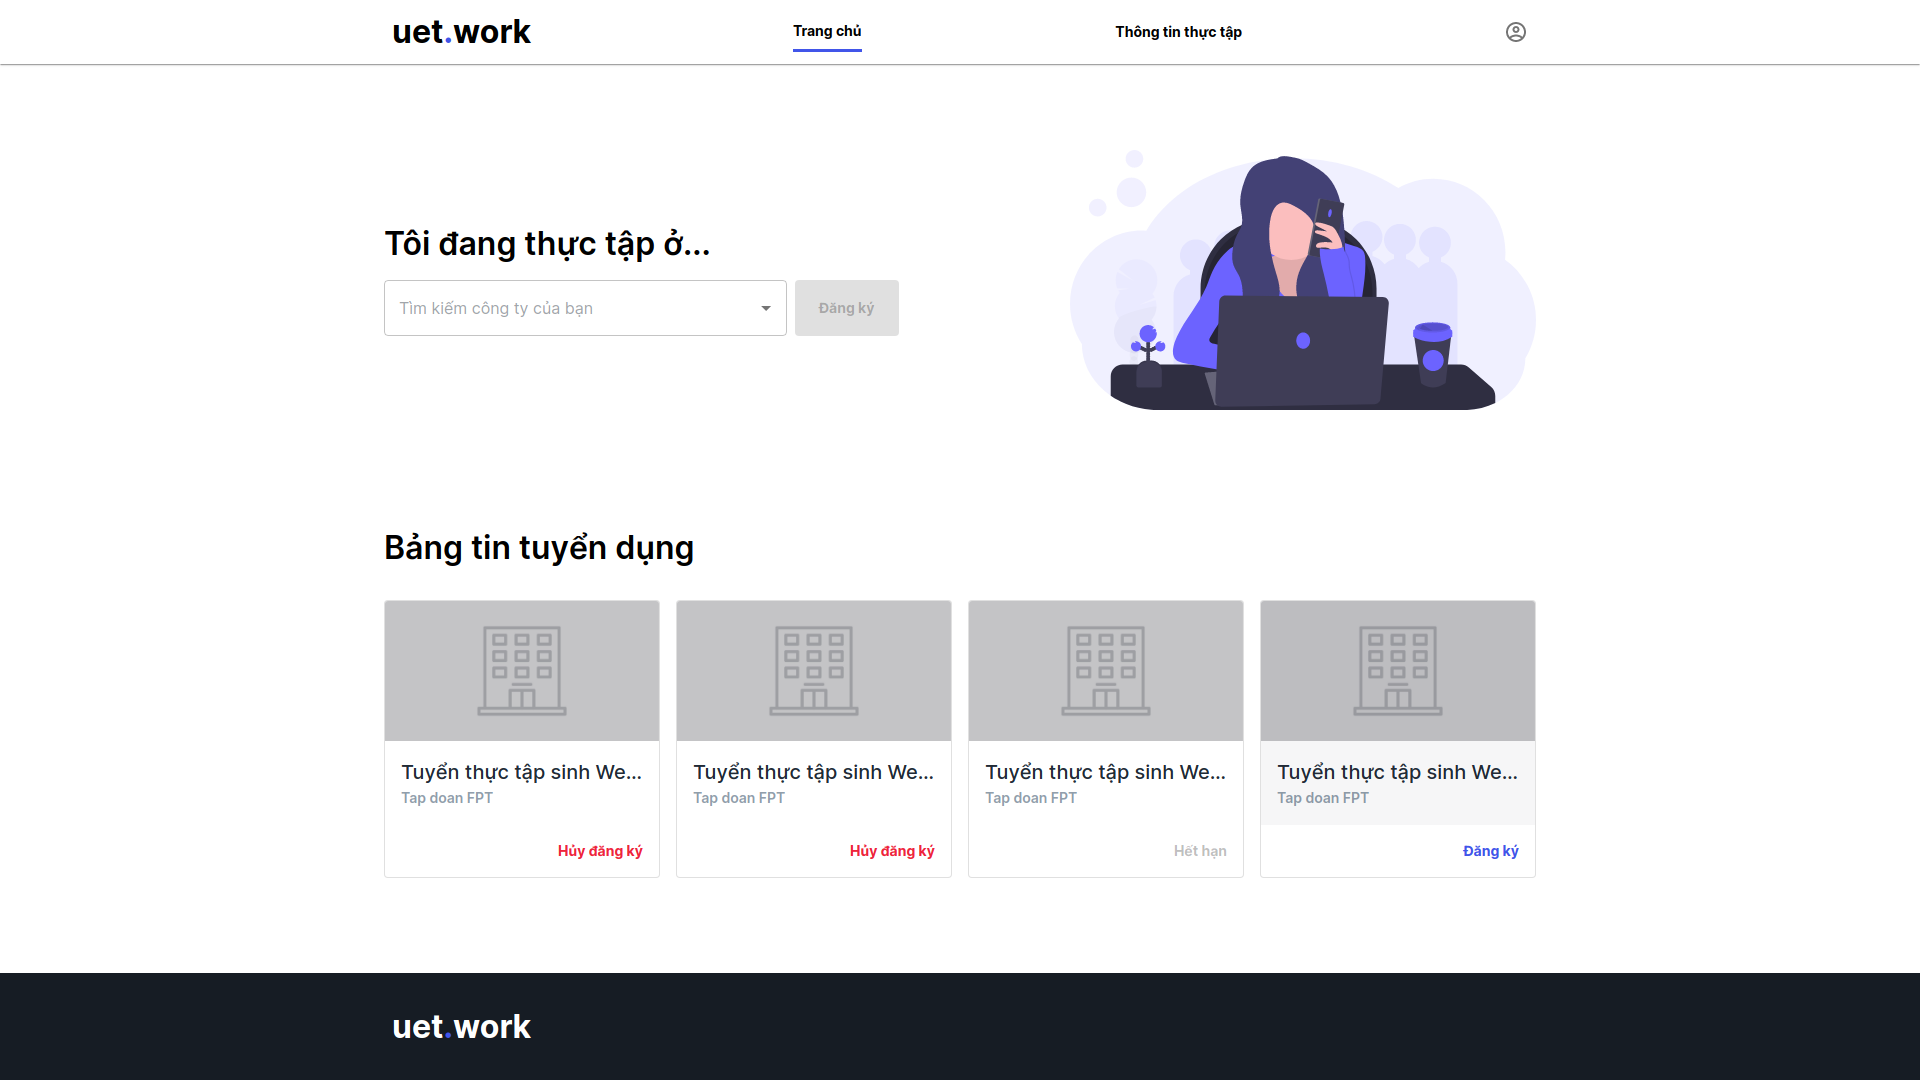
\includegraphics[width=\linewidth]{./images/image37.png}
	\caption{Luồng \emph{Đọc bài đăng}: Truy cập trang chủ và chọn bài đăng muốn đọc}
	\label{fig:student_home_page}
\end{figure}

\begin{figure}[]
	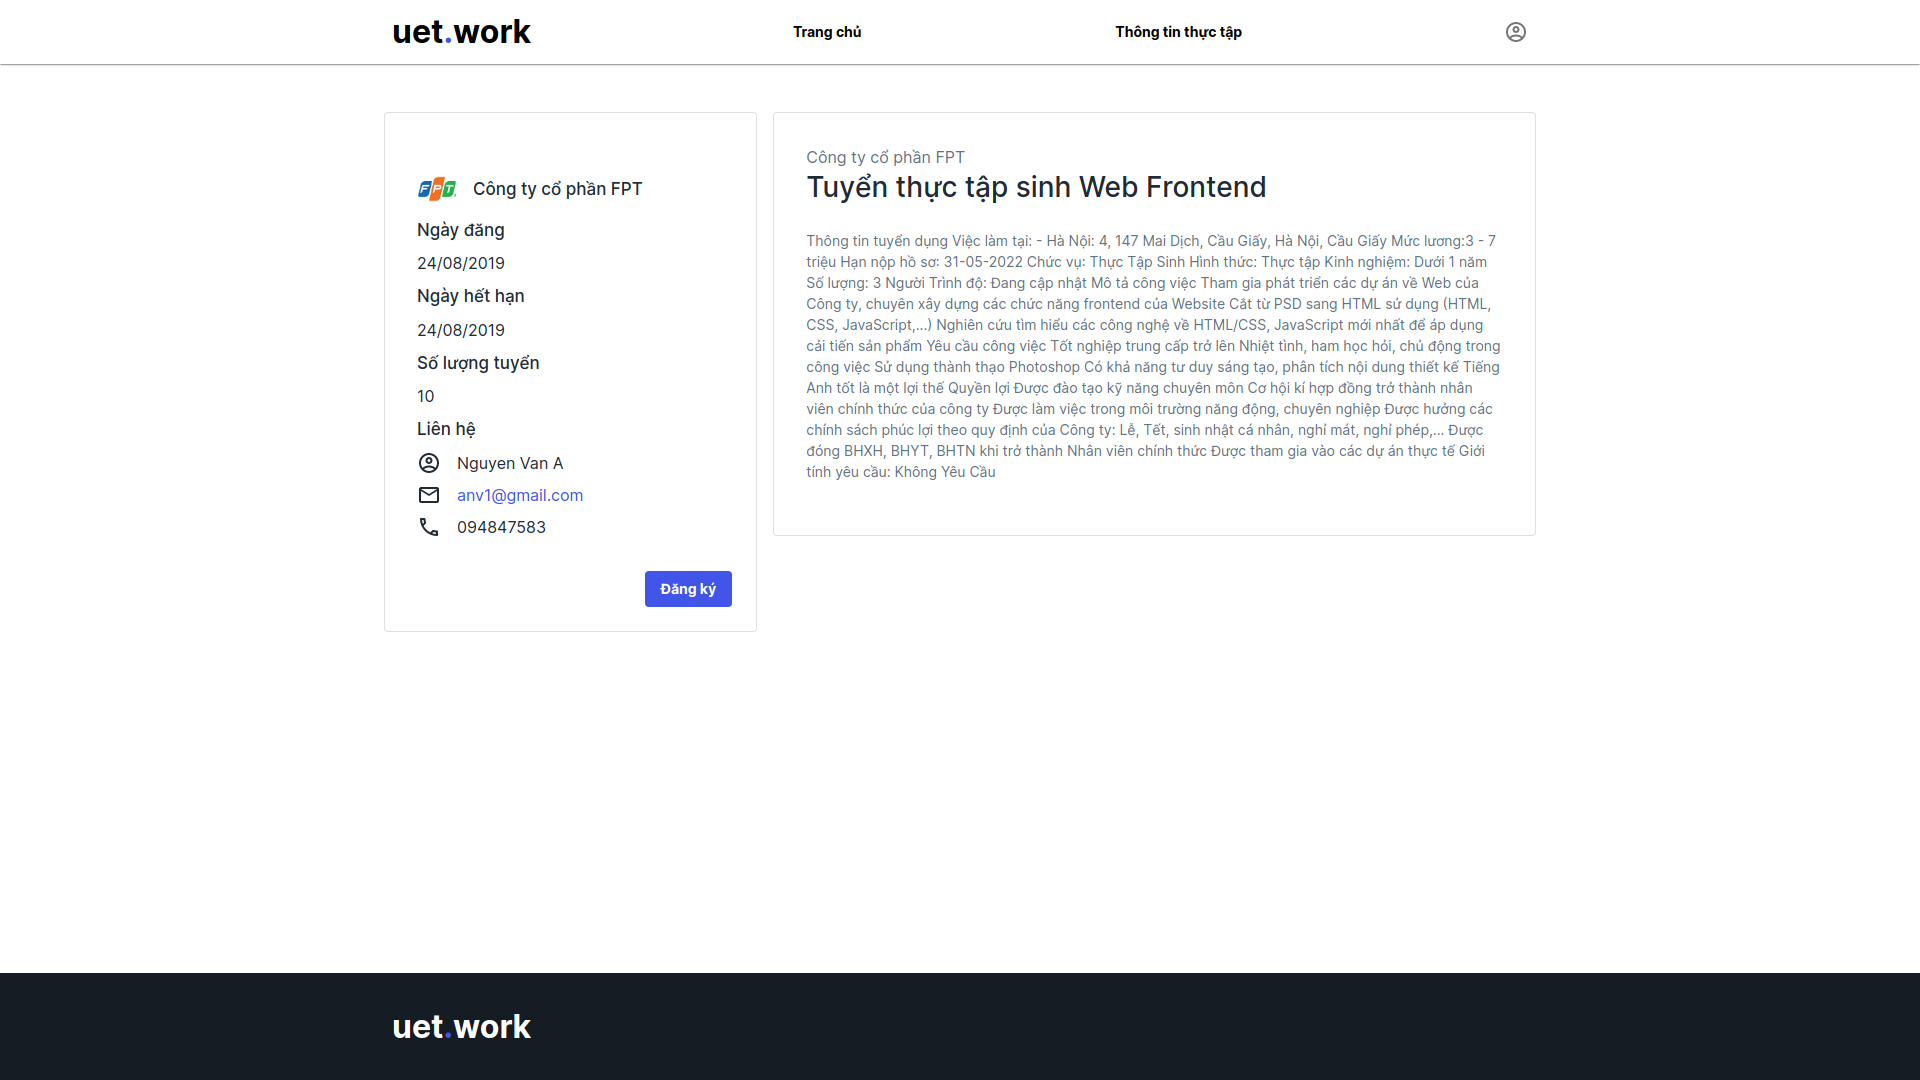
\includegraphics[width=\linewidth]{./images/image81.png}
	\caption{Luồng \emph{Đọc bài đăng}: Giao diện hiển thị bài đăng đã chọn}
	\label{fig:student_read_post_page}
\end{figure}

\paragraph*{Sinh viên đăng ký thực tập}

\begin{itemize}
	\item Hình \ref{fig:student_find_company}: Sinh viên tìm kiếm công ty mà mình đang thực tập và đăng ký.
	\item Hình \ref{fig:student_register_company_success}: Nếu thành công, hệ thống hiển thị thông báo đăng ký thành công.
	\item Hình \ref{fig:student_register_company_failed}: Nếu thất bại, hệ thống hiển thị thông báo đăng ký thất bại.
\end{itemize}

\begin{figure}[]
	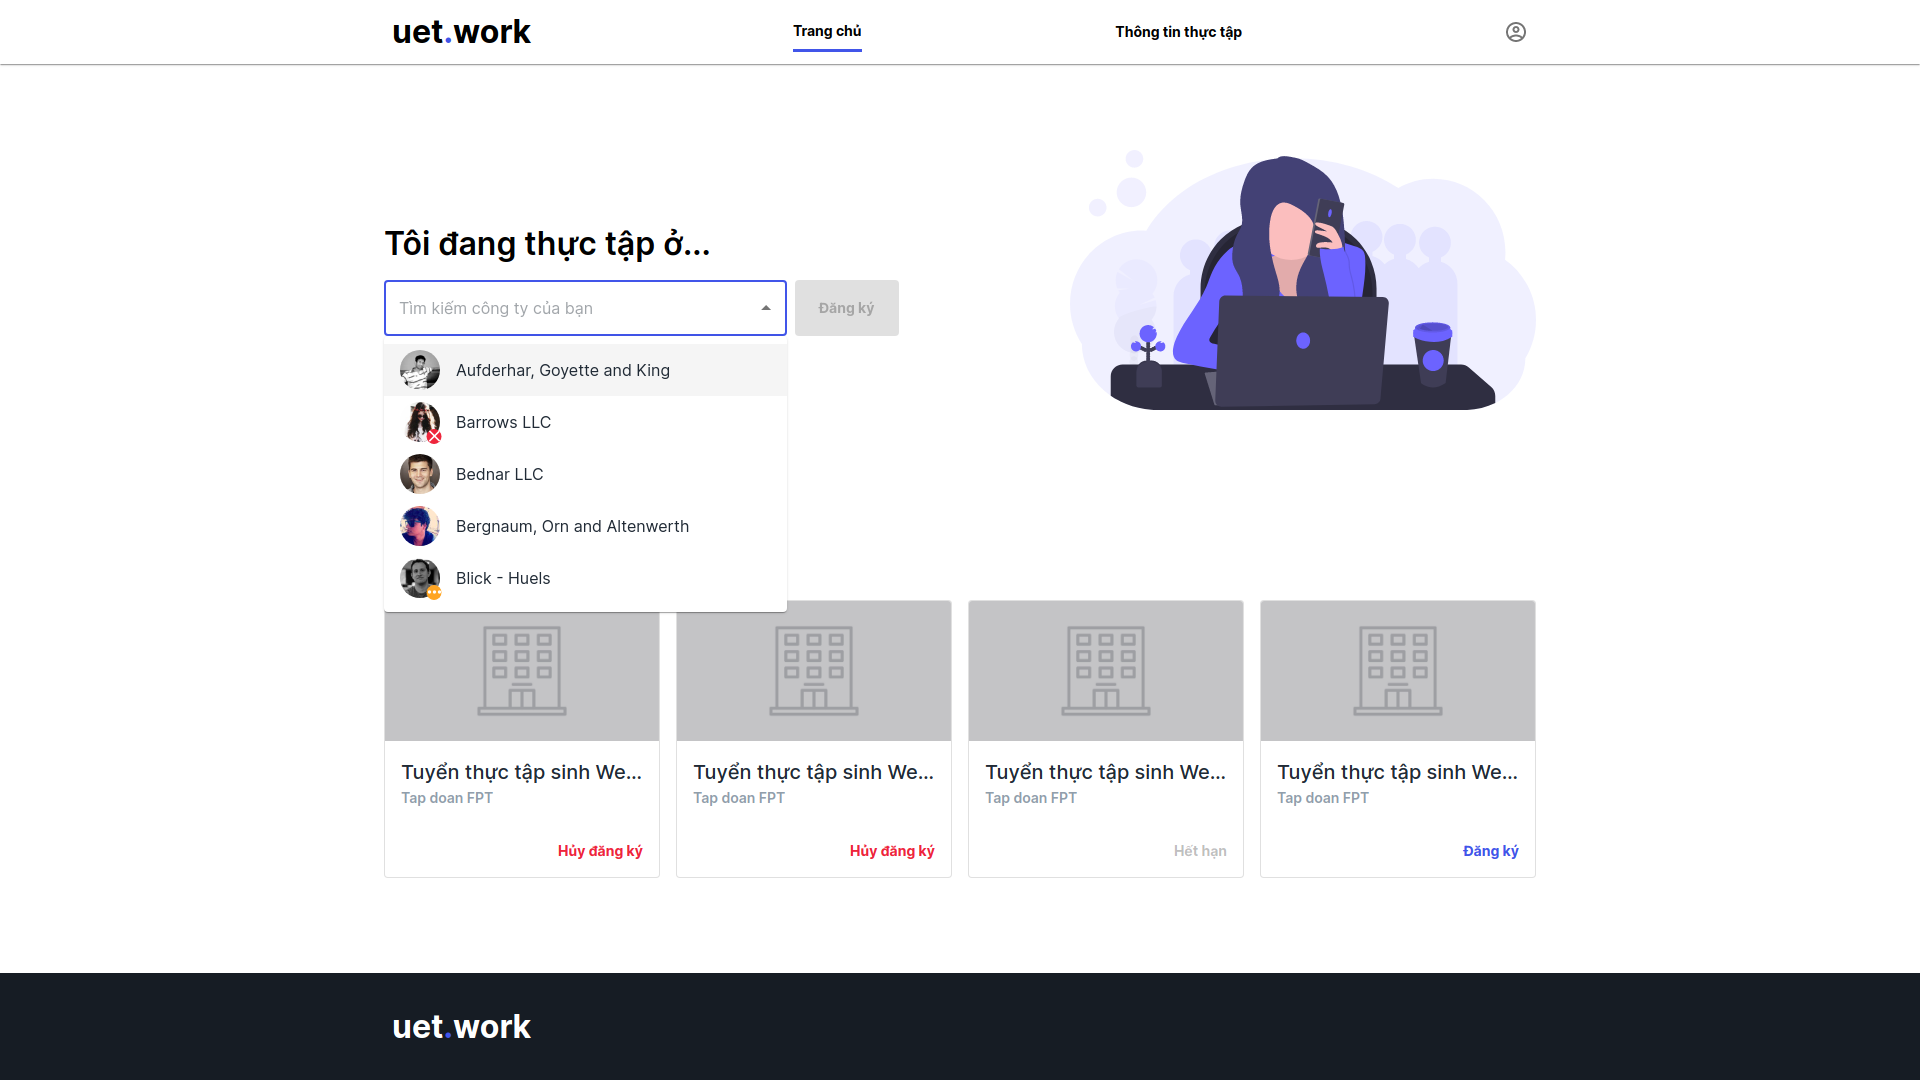
\includegraphics[width=\linewidth]{./images/image39.png}
	\caption{Luồng \emph{Sinh viên đăng ký thực tập}: Tìm kiếm công ty}
	\label{fig:student_find_company}
\end{figure}

\begin{figure}[]
	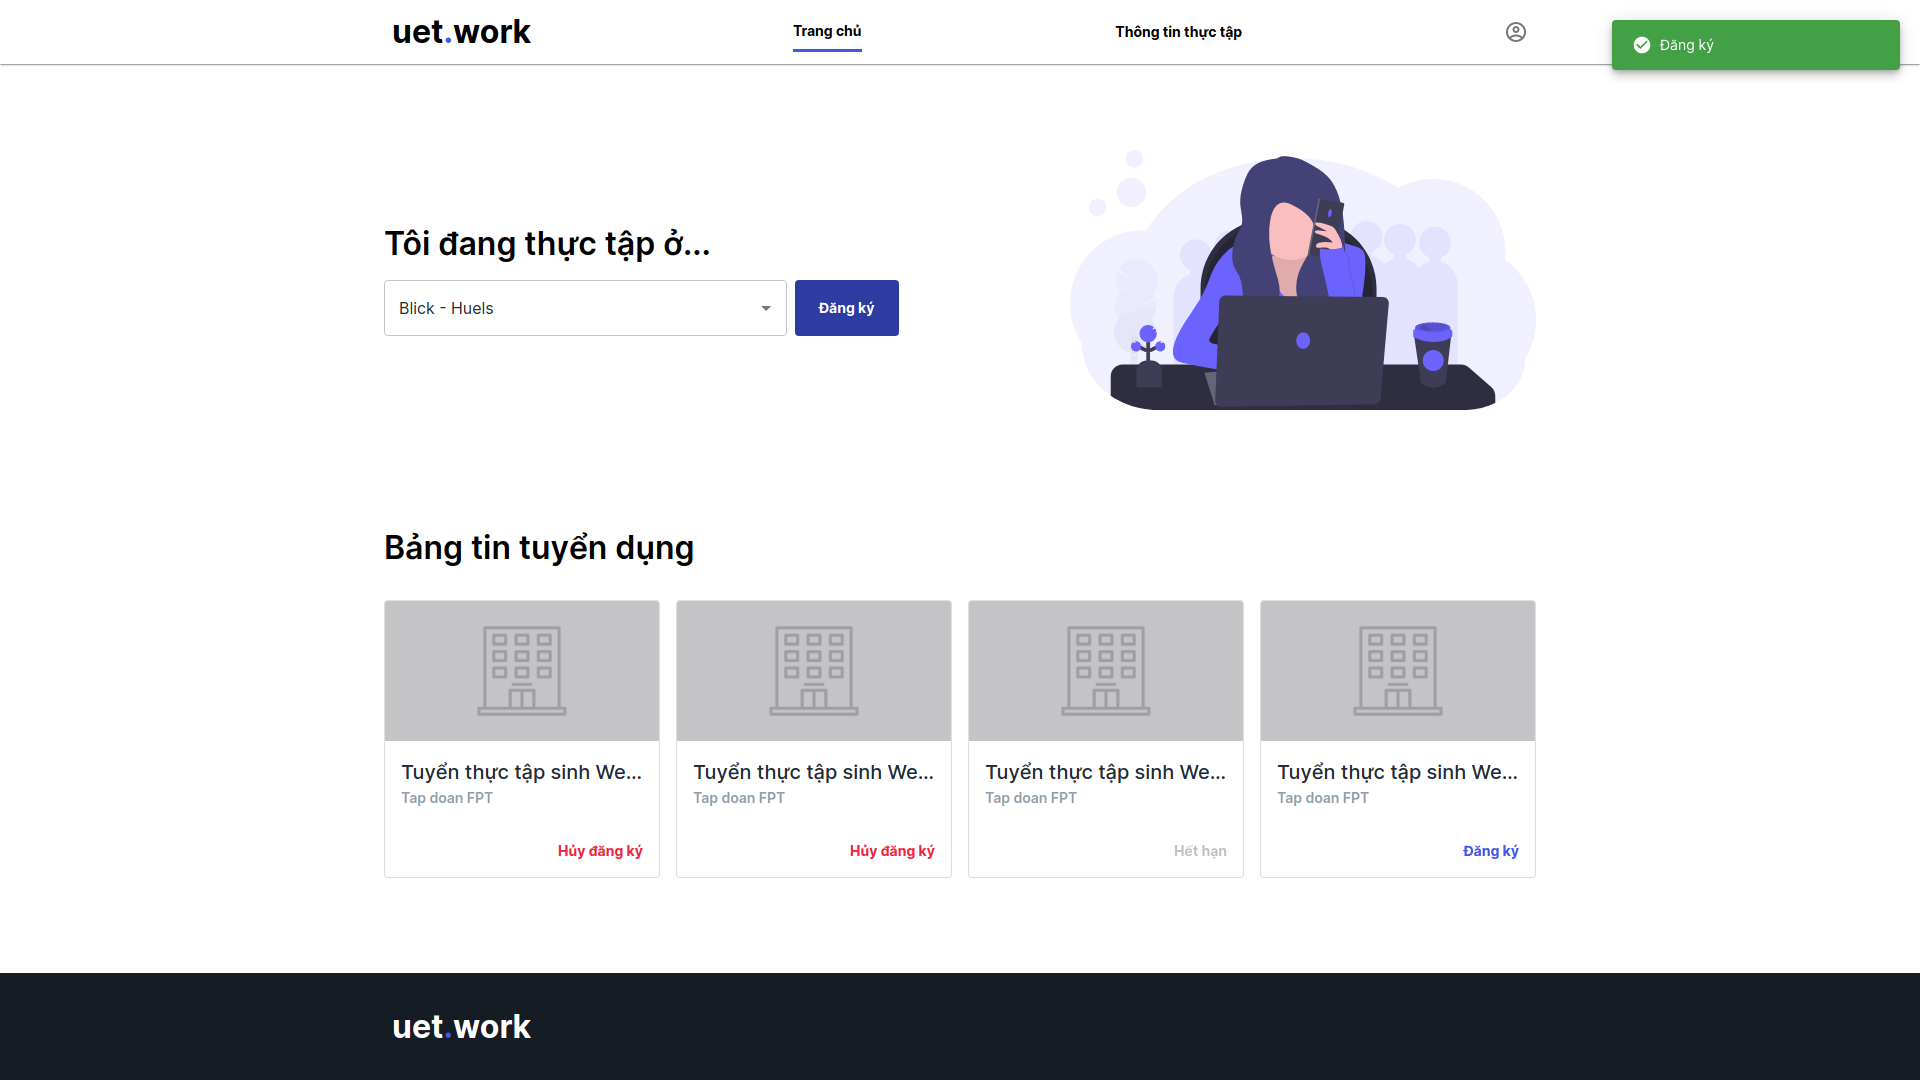
\includegraphics[width=\linewidth]{./images/image40-1.png}
	\caption{Luồng \emph{Sinh viên đăng ký thực tập}: Đăng ký thành công}
	\label{fig:student_register_company_success}
\end{figure}

\begin{figure}[]
	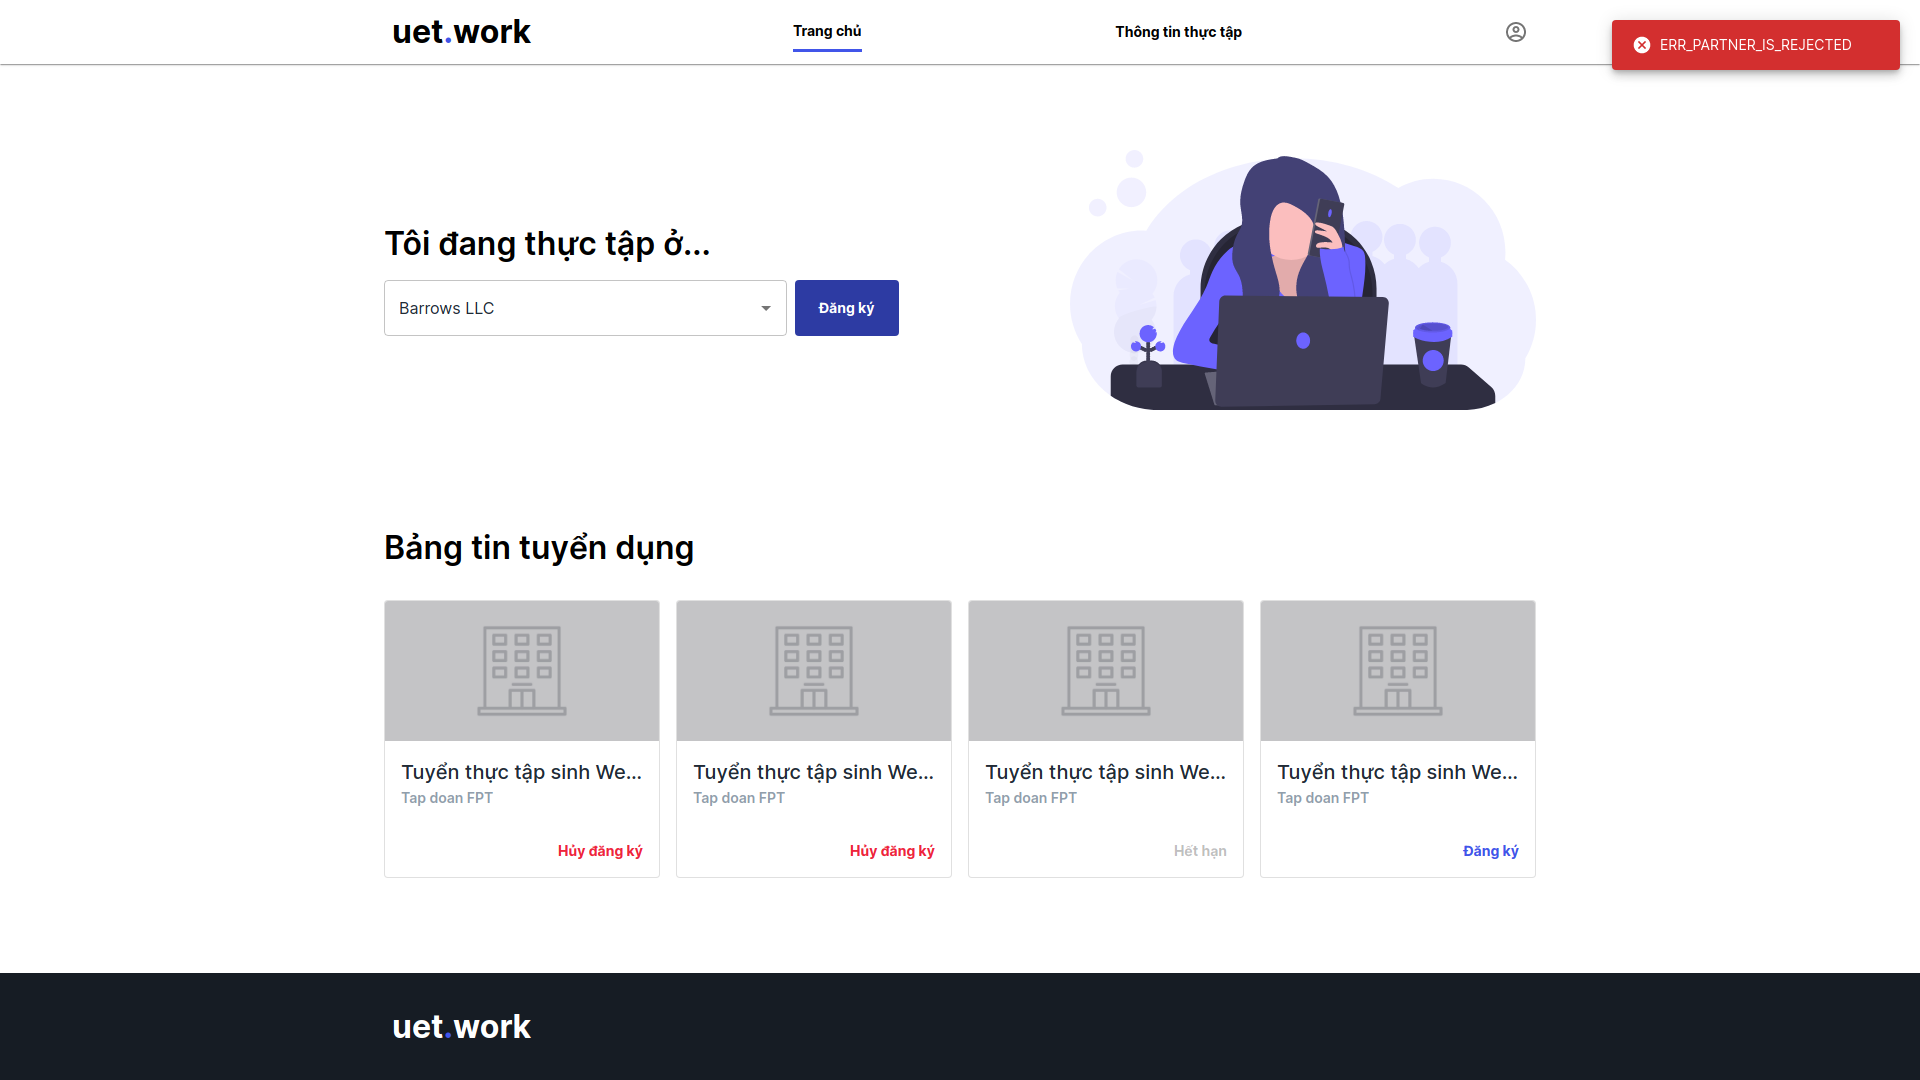
\includegraphics[width=\linewidth]{./images/image40.png}
	\caption{Luồng \emph{Sinh viên đăng ký thực tập}: Đăng ký thất bại}
	\label{fig:student_register_company_failed}
\end{figure}

\paragraph*{Sinh viên xem thông tin thực tập}
Sau khi đăng ký thực tập thành công, sinh viên vào kiểm tra thông tin thực tập của bản thân. Tại đây, sinh viên có thể xem thông tin công ty thực tập đã đúng chưa, giảng viên hướng dẫn là ai, và nộp báo cáo.

Hình \ref{fig:view_internship_page} mô tả màn hình trang thông tin thực tập.

\begin{figure}[]
	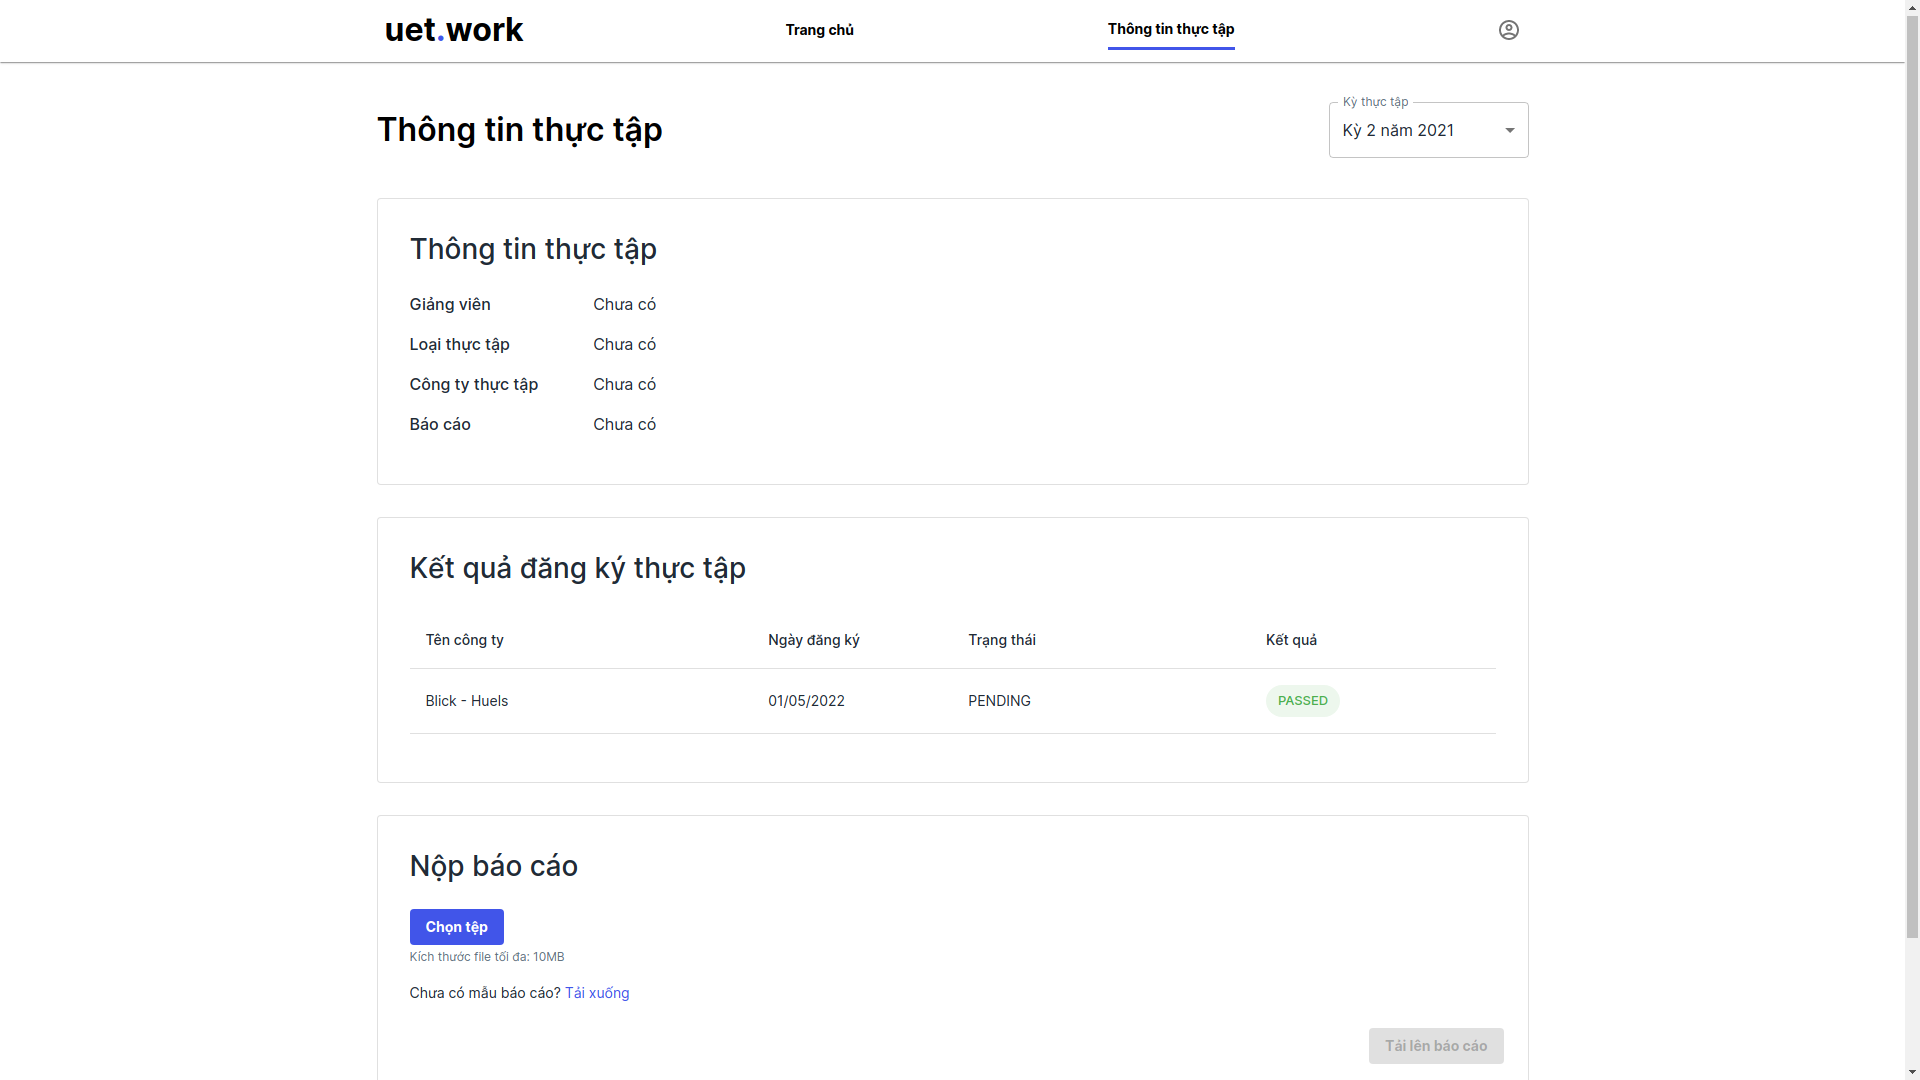
\includegraphics[width=\linewidth]{./images/image17.png}
	\caption{Luồng \emph{Sinh viên xem thông tin thực tập}}
	\label{fig:view_internship_page}
\end{figure}

\paragraph*{Sinh viên nộp báo cáo thực tập}

\begin{itemize}
	\item Hình \ref{fig:student_internship_info}: Sinh viên truy cập trang thông tin thực tập và kéo xuống phần Nộp báo cáo.
	\item Hình \ref{fig:student_choose_file}: Sinh viên chọn tệp.
	\item Hình \ref{fig:student_upload_report}: Sinh viên tải lên báo cáo.
\end{itemize}

\begin{figure}[]
	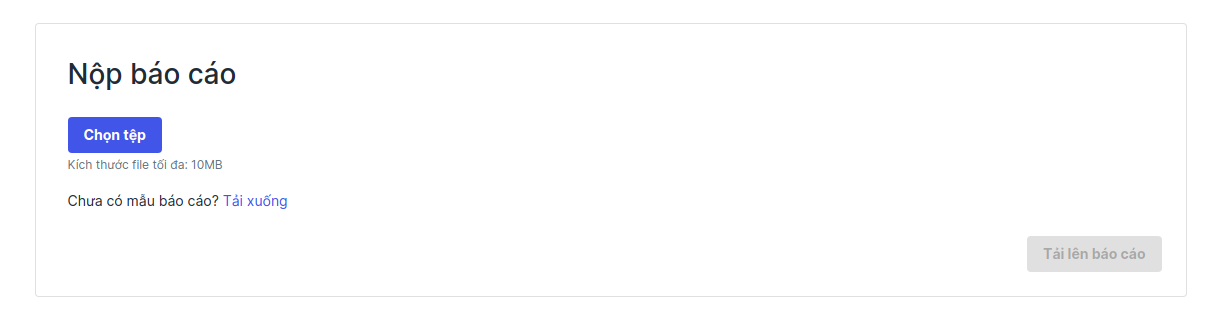
\includegraphics[width=\linewidth]{./images/image41.png}
	\caption{Luồng \emph{Sinh viên nộp báo cáo}: Truy cập phần nộp báo cáo}
	\label{fig:student_internship_info}
\end{figure}

\begin{figure}[]
	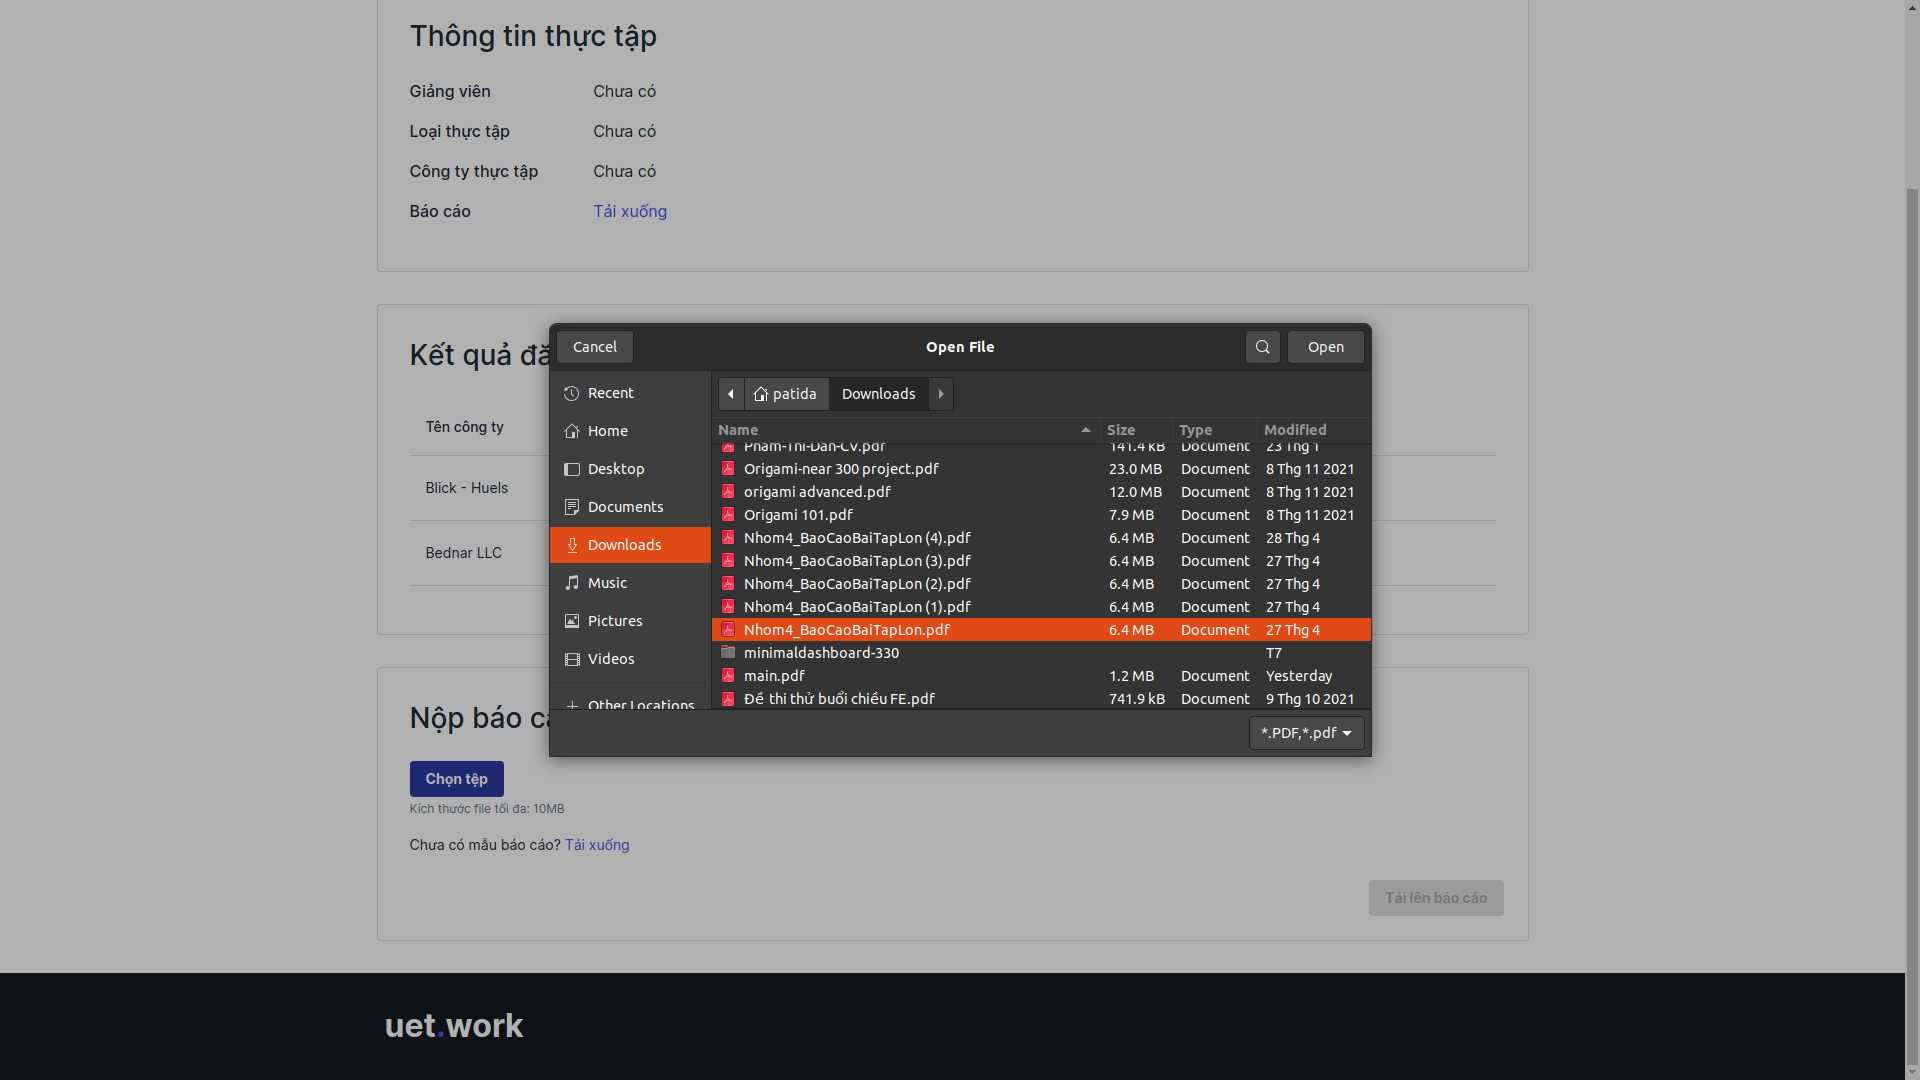
\includegraphics[width=\linewidth]{./images/image42.png}
	\caption{Luồng \emph{Sinh viên nộp báo cáo}: Chọn tệp}
	\label{fig:student_choose_file}
\end{figure}

\begin{figure}[]
	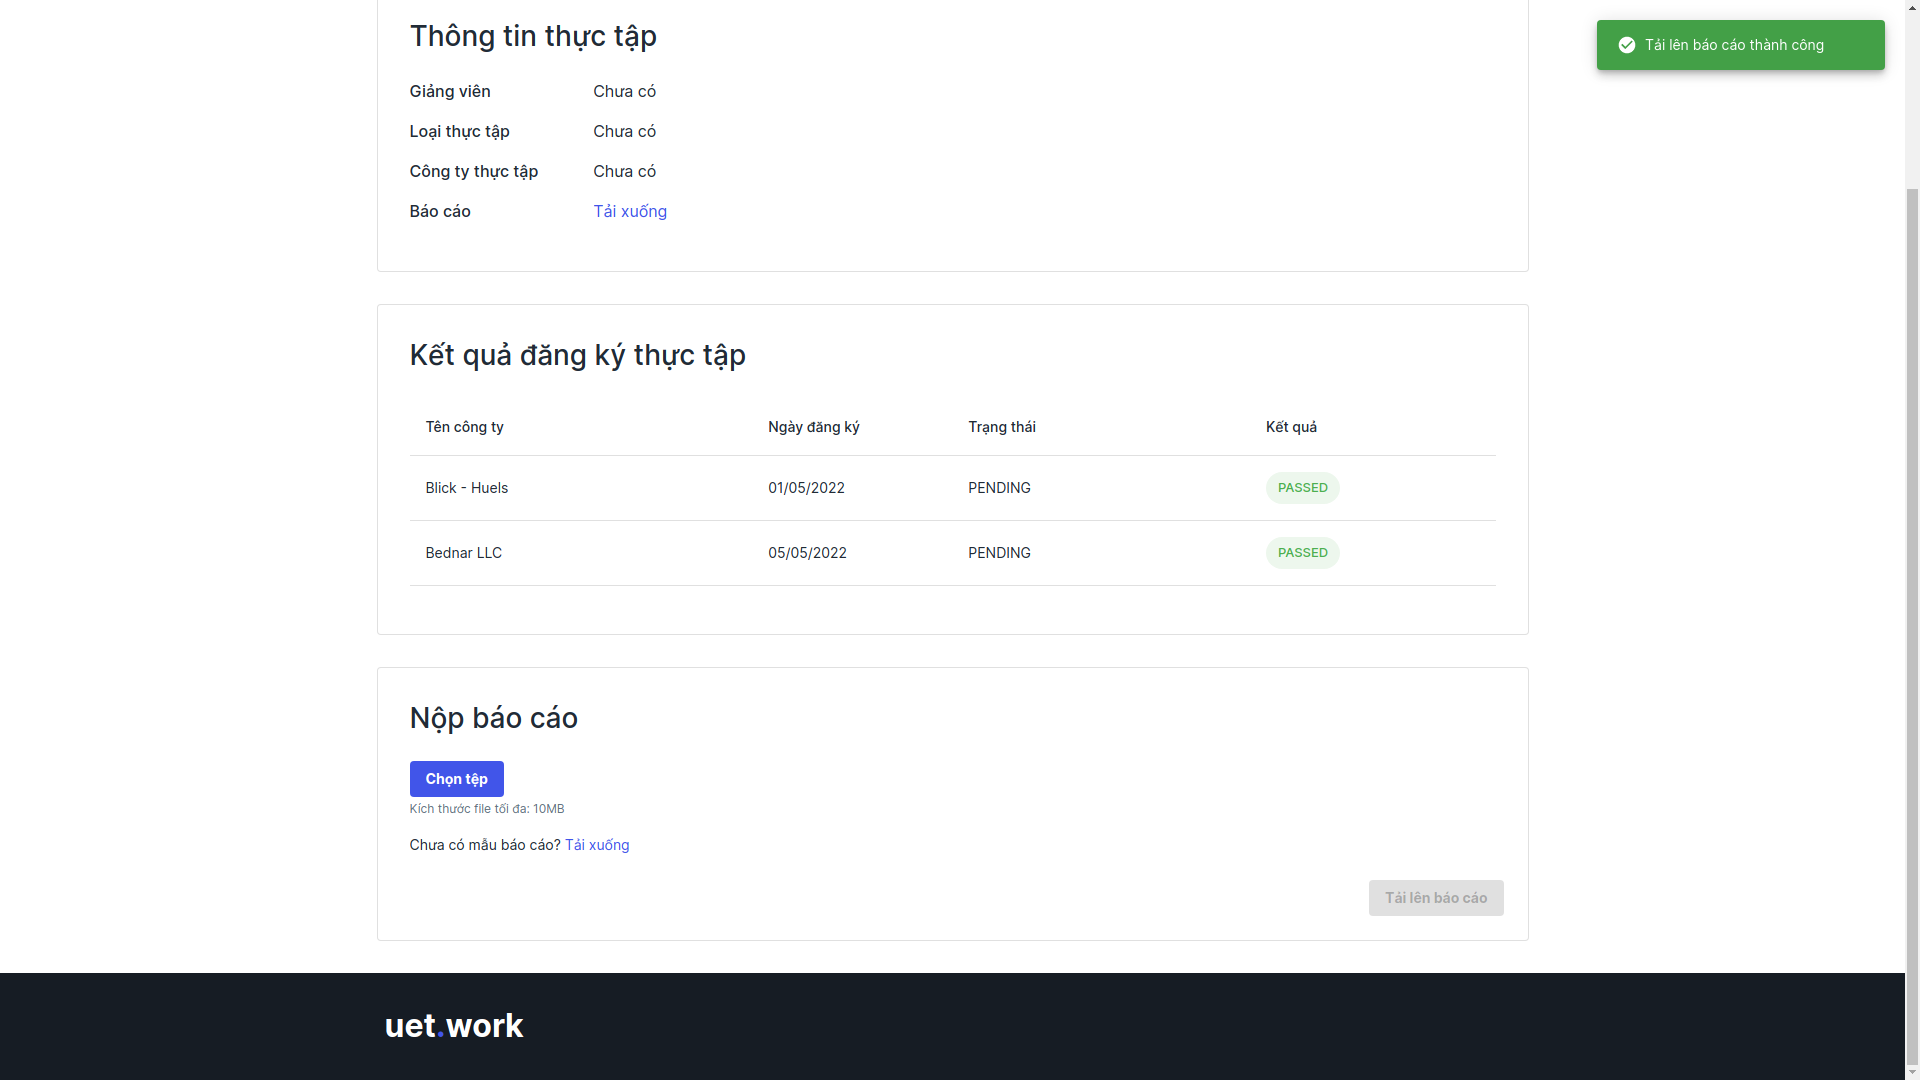
\includegraphics[width=\linewidth]{./images/image43.png}
	\caption{Luồng \emph{Sinh viên nộp báo cáo}: Tải lên báo cáo}
	\label{fig:student_upload_report}
\end{figure}

\paragraph*{Sinh viên xem thông tin cá nhân}
Sinh viên truy cập trang thông tin cá nhân. Tại đây sinh viên có thể sửa thông tin cá nhân, đổi mật khẩu.

Hình \ref{fig:view_info_page} mô tả màn hình trang thông tin cá nhân.

\begin{figure}[]
	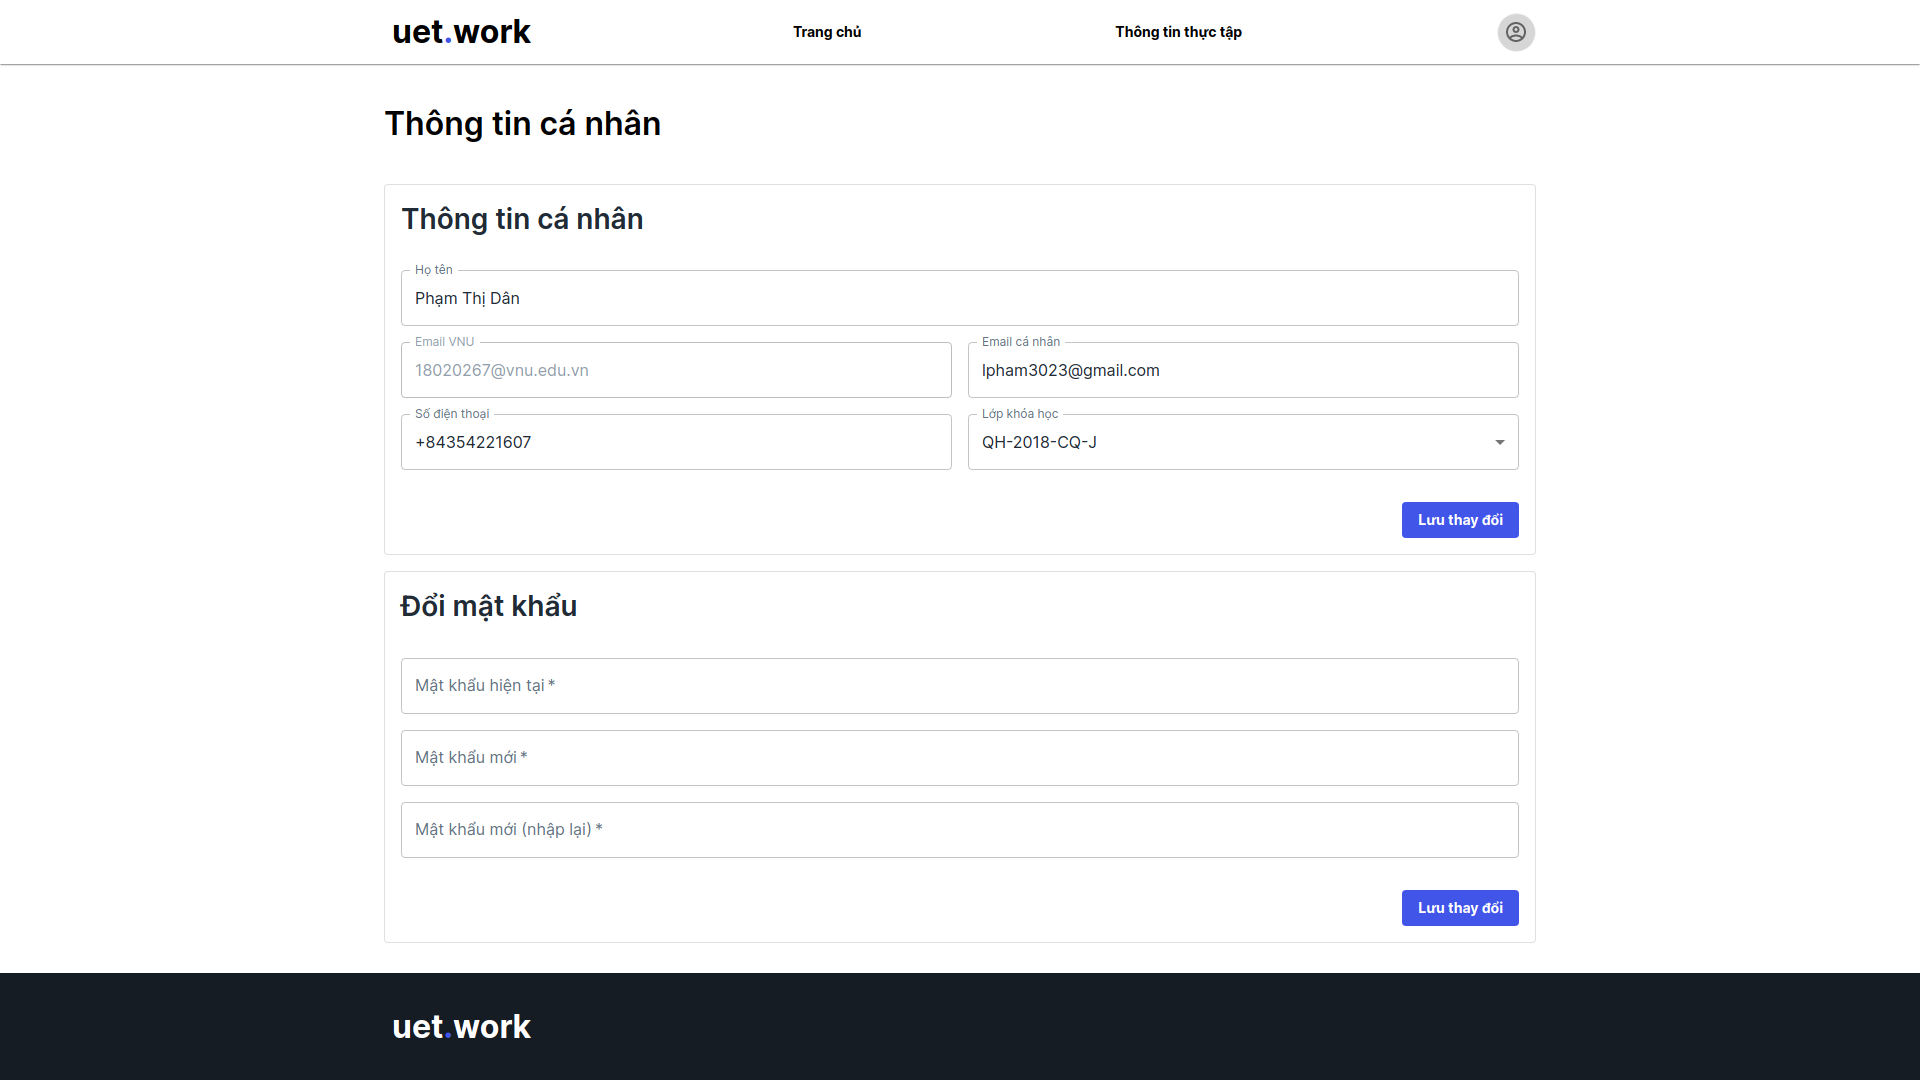
\includegraphics[width=\linewidth]{./images/image44.png}
	\caption{Luồng \emph{Sinh viên xem thông tin cá nhân}}
	\label{fig:view_info_page}
\end{figure}

\paragraph*{Sinh viên thay đổi thông tin cá nhân}

\begin{itemize}
	\item Hình \ref{fig:student_access_info}: Sinh viên truy cập phần thông tin cá nhân.
	\item Hình \ref{fig:student_edit_info}: Sinh viên sửa thông tin cá nhân, đổi mật khẩu.
\end{itemize}

\begin{figure}[]
	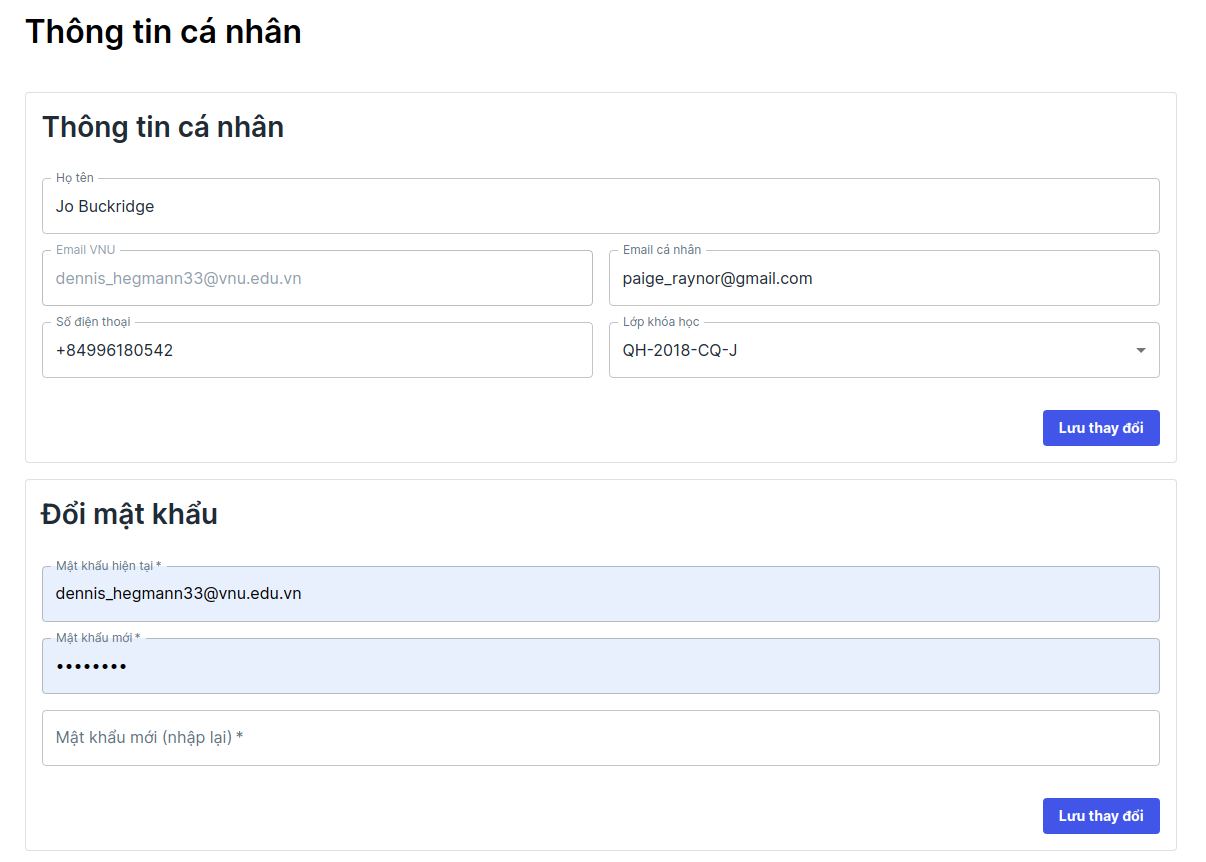
\includegraphics[width=\linewidth]{./images/image45.png}
	\caption{Luồng \emph{Sinh viên thay đổi thông tin cá nhân}: Truy cập trang thông tin cá nhân}
	\label{fig:student_access_info}
\end{figure}

\begin{figure}[]
	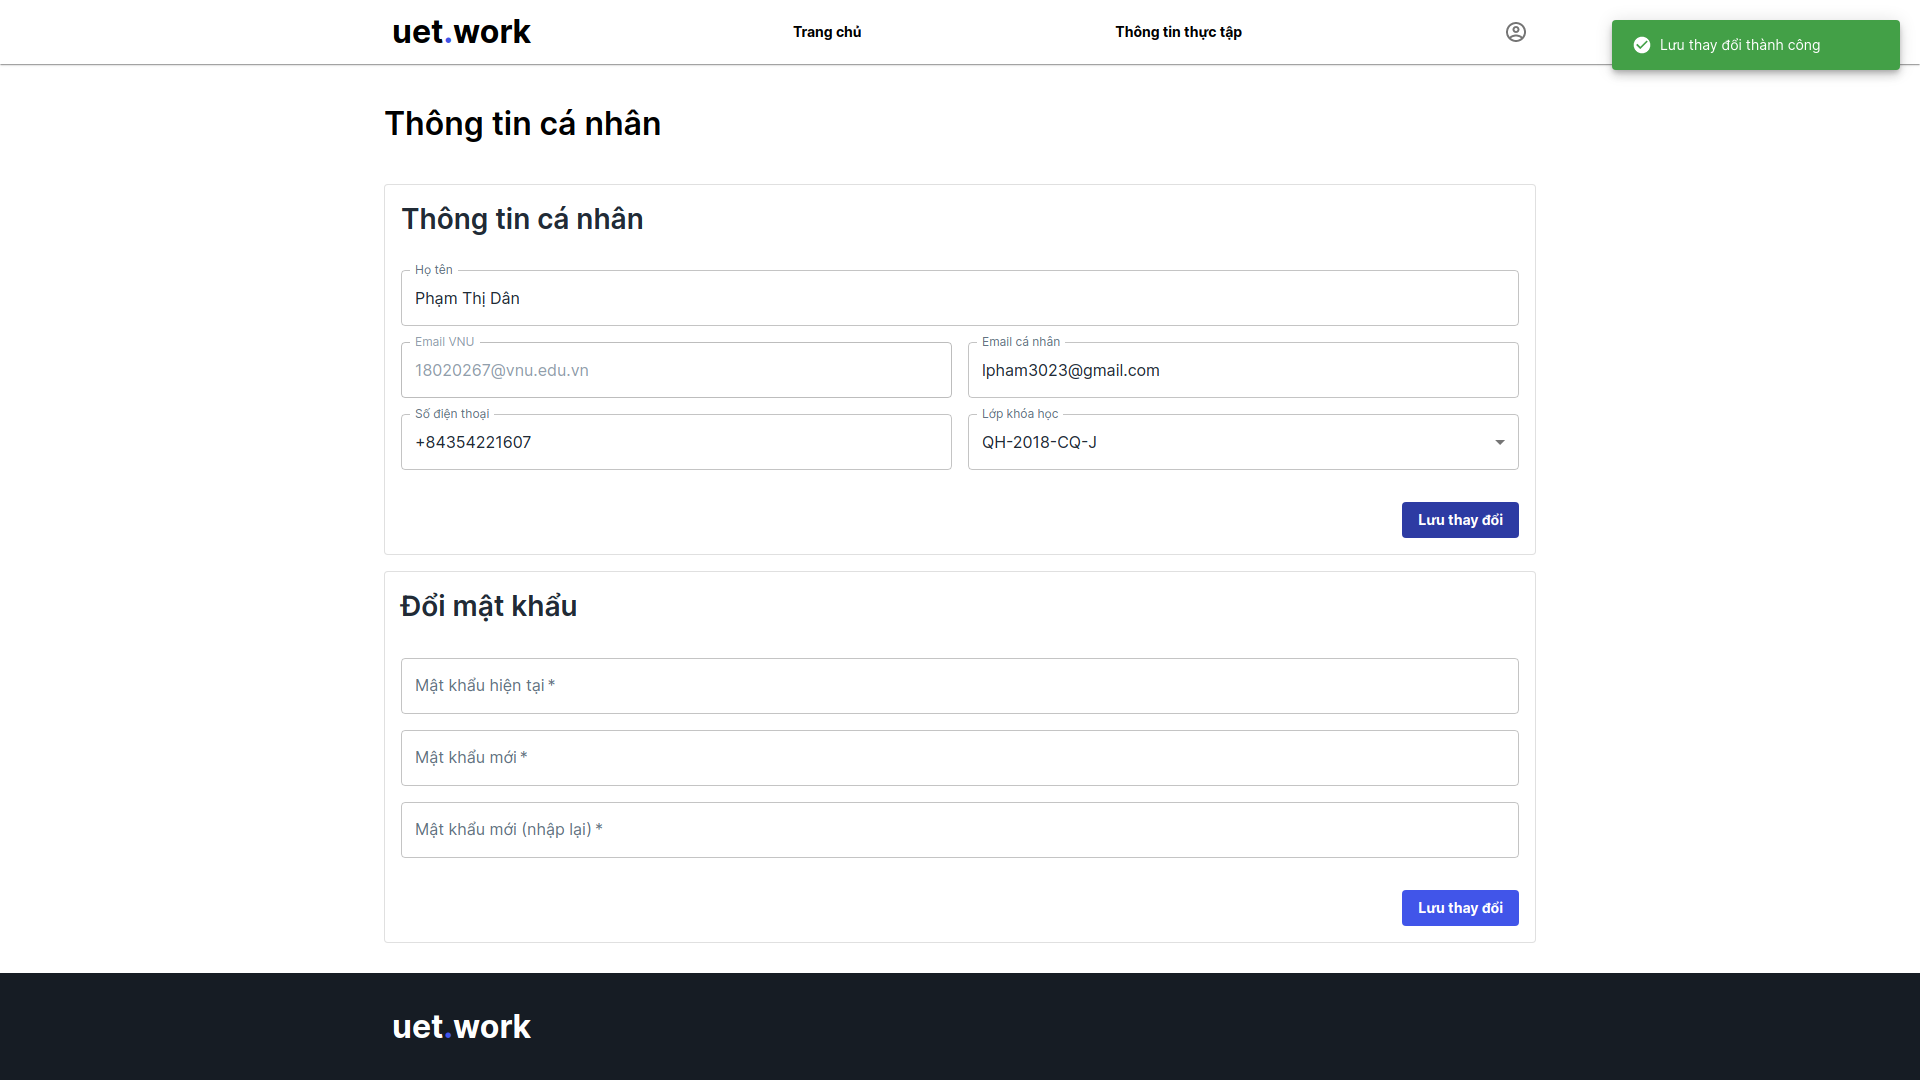
\includegraphics[width=\linewidth]{./images/image46.png}
	\caption{Luồng \emph{Sinh viên thay đổi thông tin cá nhân}: Sinh viên thay đổi thông tin cá nhân}
	\label{fig:student_edit_info}
\end{figure}

\subsubsection{Luồng sử dụng của giảng viên}

\paragraph*{Giảng viên xem danh sách sinh viên đang hướng dẫn}

Giảng viên truy cập trang Sinh viên đang hướng dẫn. Tại đây, giảng viên có thể tìm kiếm, sắp xếp, lọc danh sách theo kỳ thực tập, trạng thái báo cáo, trạng thái chấm điểm.

Hình \ref{fig:working_student_page} mô tả màn hình danh sách sinh viên đang hướng dẫn.

\begin{figure}[]
	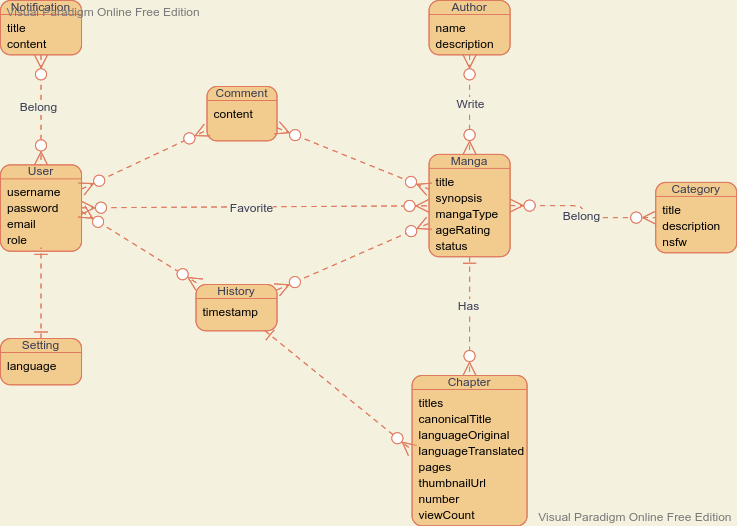
\includegraphics[width=\linewidth]{./images/image8.png}
	\caption{Luồng \emph{Giảng viên xem danh sách sinh viên đang hướng dẫn}}
	\label{fig:working_student_page}
\end{figure}

\paragraph*{Giảng viên tải xuống báo cáo}
Hình \ref{fig:lecturer_access_students}: Giảng viên truy cập trang sinh viên đang hướng dẫn và tải xuống báo cáo của sinh viên.

\begin{figure}[]
	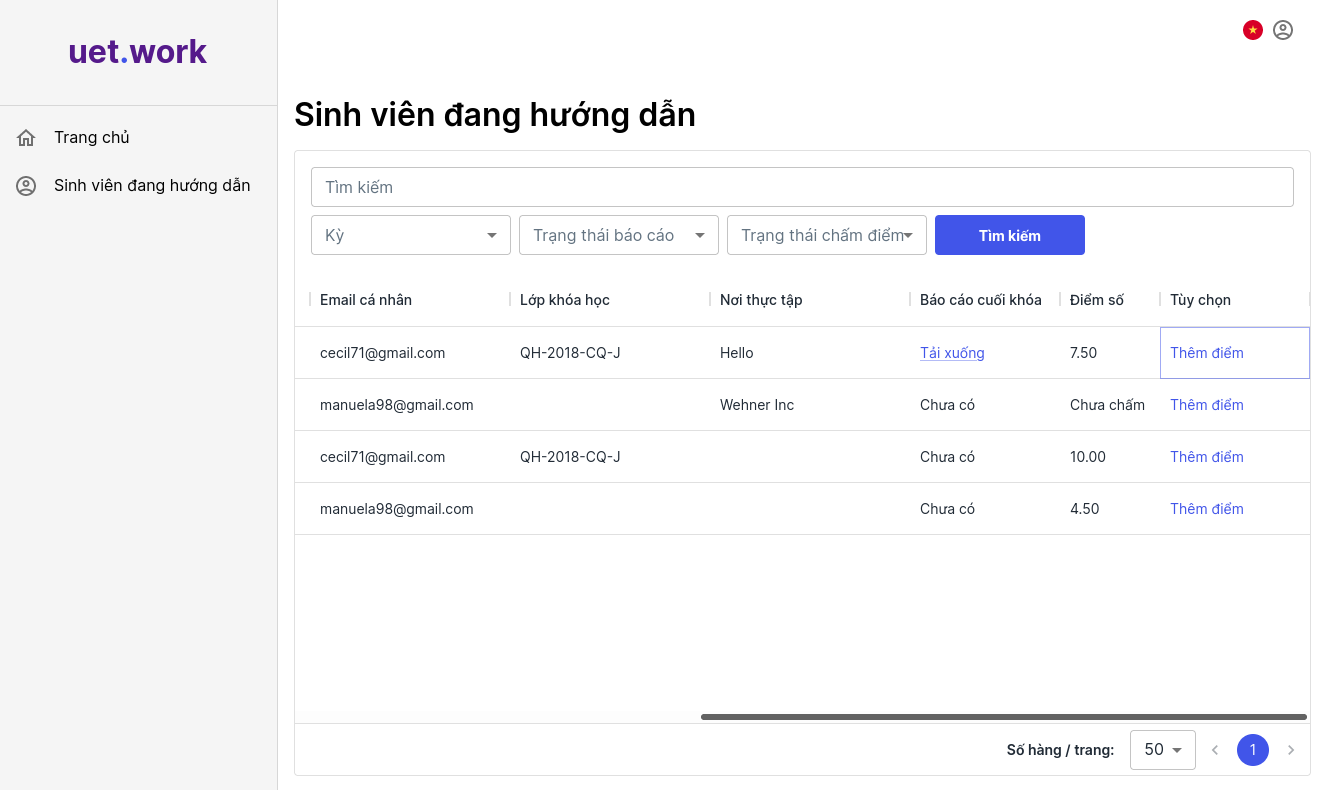
\includegraphics[width=\linewidth]{./images/image64.png}
	\caption{Luồng \emph{Giảng viên tải xuống báo cáo}}
	\label{fig:lecturer_access_students}
\end{figure}

\paragraph*{Giảng viên chấm điểm cho sinh viên}

\begin{itemize}
	\item Hình \ref{fig:lecturer_access_students_page}: Giảng viên truy cập trang sinh viên đang hướng dẫn.
	\item Hình \ref{fig:lecturer_score}: Giảng viên chấm điểm cho sinh viên.
\end{itemize}

\begin{figure}[]
	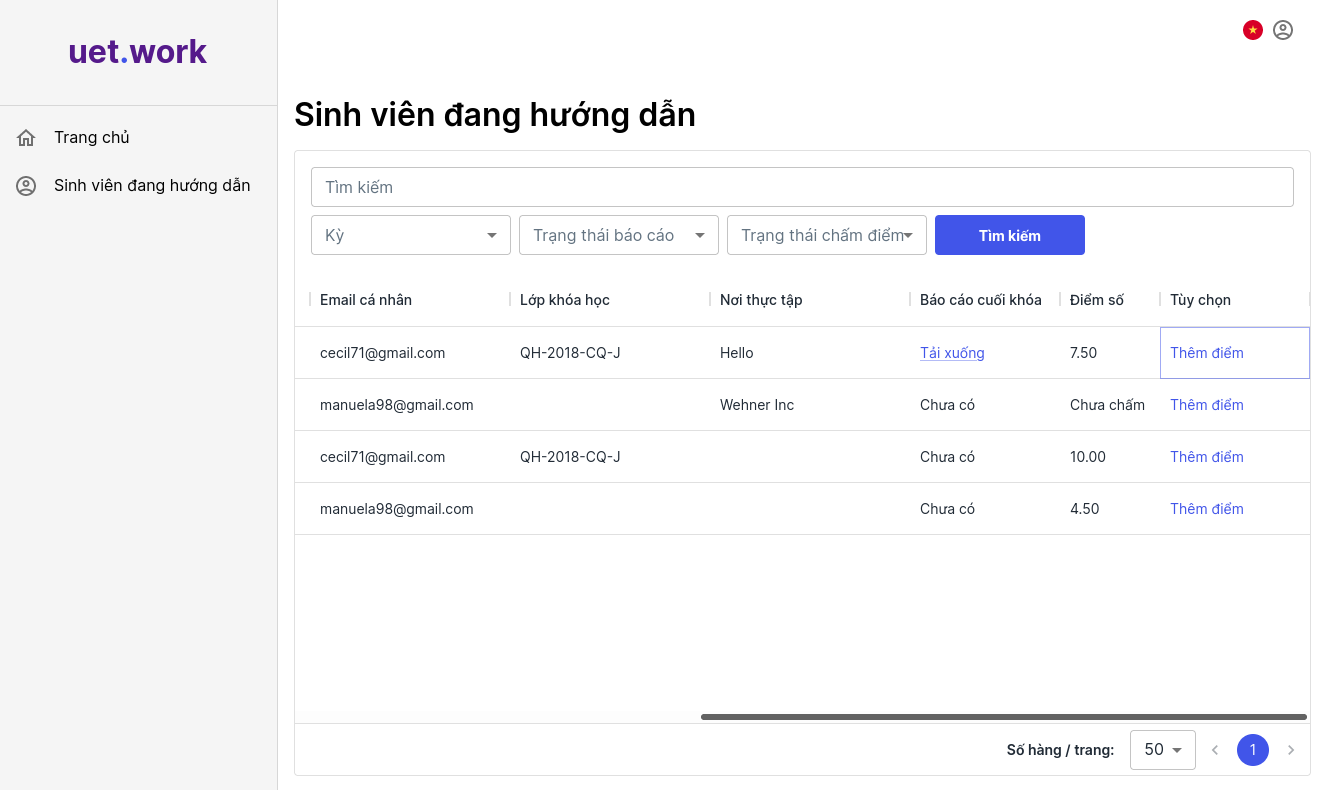
\includegraphics[width=\linewidth]{./images/image64.png}
	\caption{Luồng \emph{Giảng viên chấm điểm cho sinh viên}: Giảng viên truy cập trang sinh viên đang hướng dẫn}
	\label{fig:lecturer_access_students_page}
\end{figure}

\begin{figure}[]
	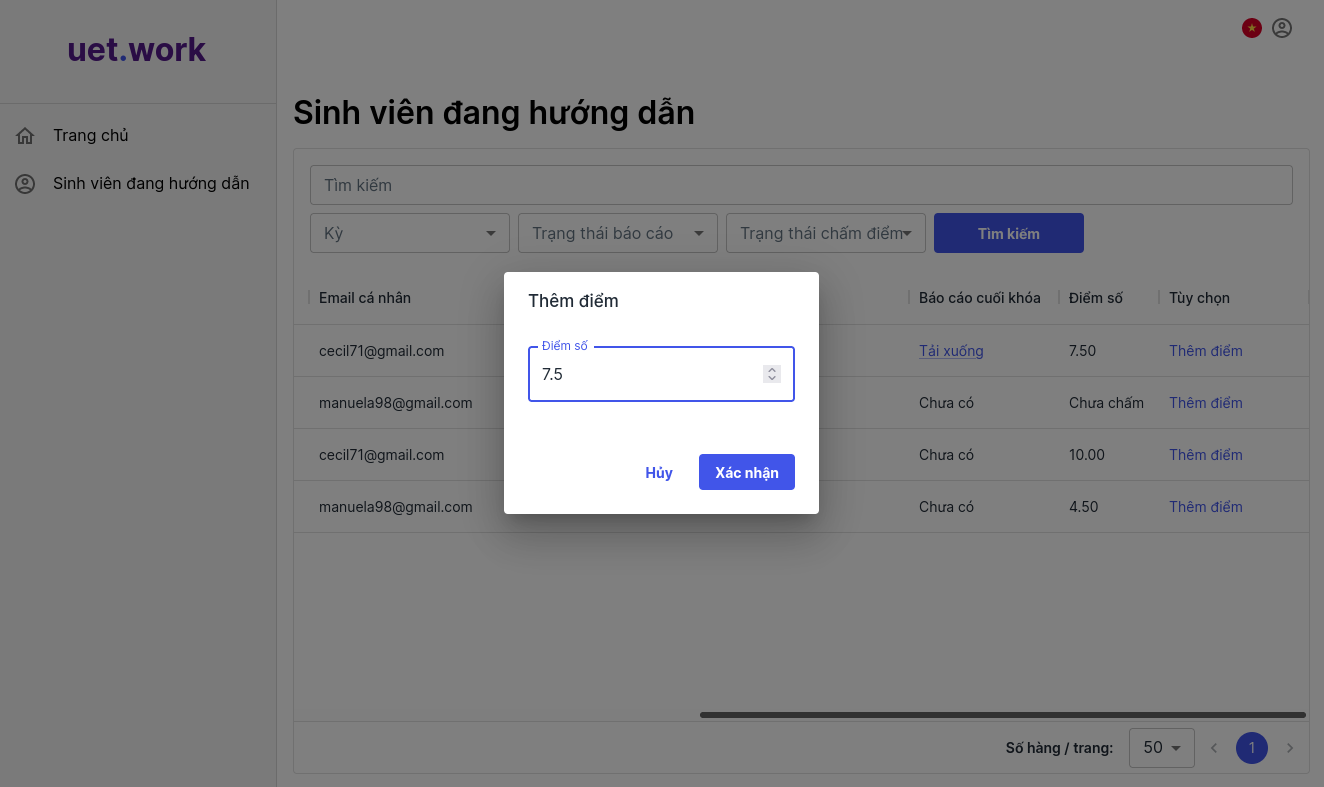
\includegraphics[width=\linewidth]{./images/image65.png}
	\caption{Luồng \emph{Giảng viên chấm điểm cho sinh viên}: Giảng viên chấm điểm cho sinh viên}
	\label{fig:lecturer_score}
\end{figure}

\paragraph*{Giảng viên thay đổi thông tin cá nhân}

\begin{itemize}
	\item Hình \ref{fig:lecturer_access_info_page}: Giảng viên truy cập trang thông tin cá nhân.
	\item Hình \ref{fig:lecturer_edit_info}: Giảng viên thay đổi thông tin cá nhân.
\end{itemize}

\begin{figure}[]
	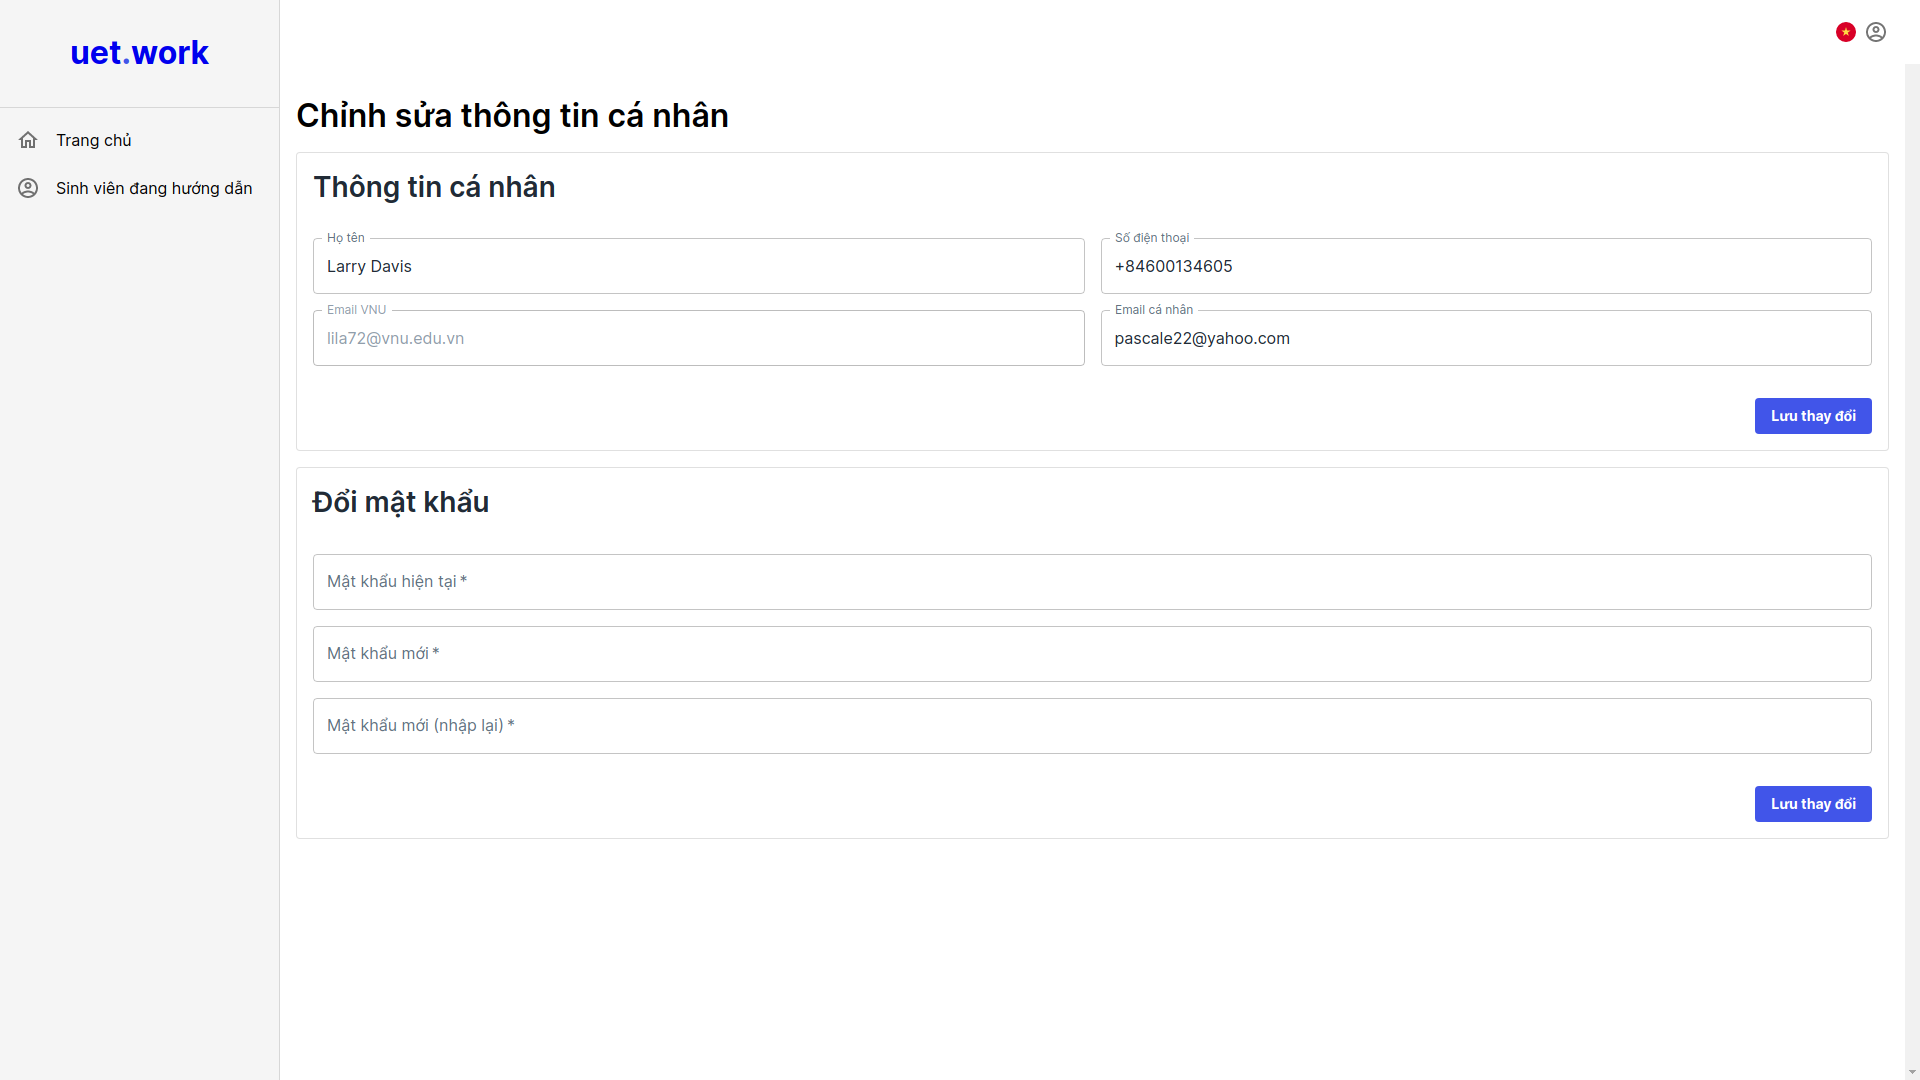
\includegraphics[width=\linewidth]{./images/image51.png}
	\caption{Luồng \emph{Giảng viên thay đổi thông tin cá nhân}: Giảng viên truy cập trang thông tin cá nhân}
	\label{fig:lecturer_access_info_page}
\end{figure}

\begin{figure}[]
	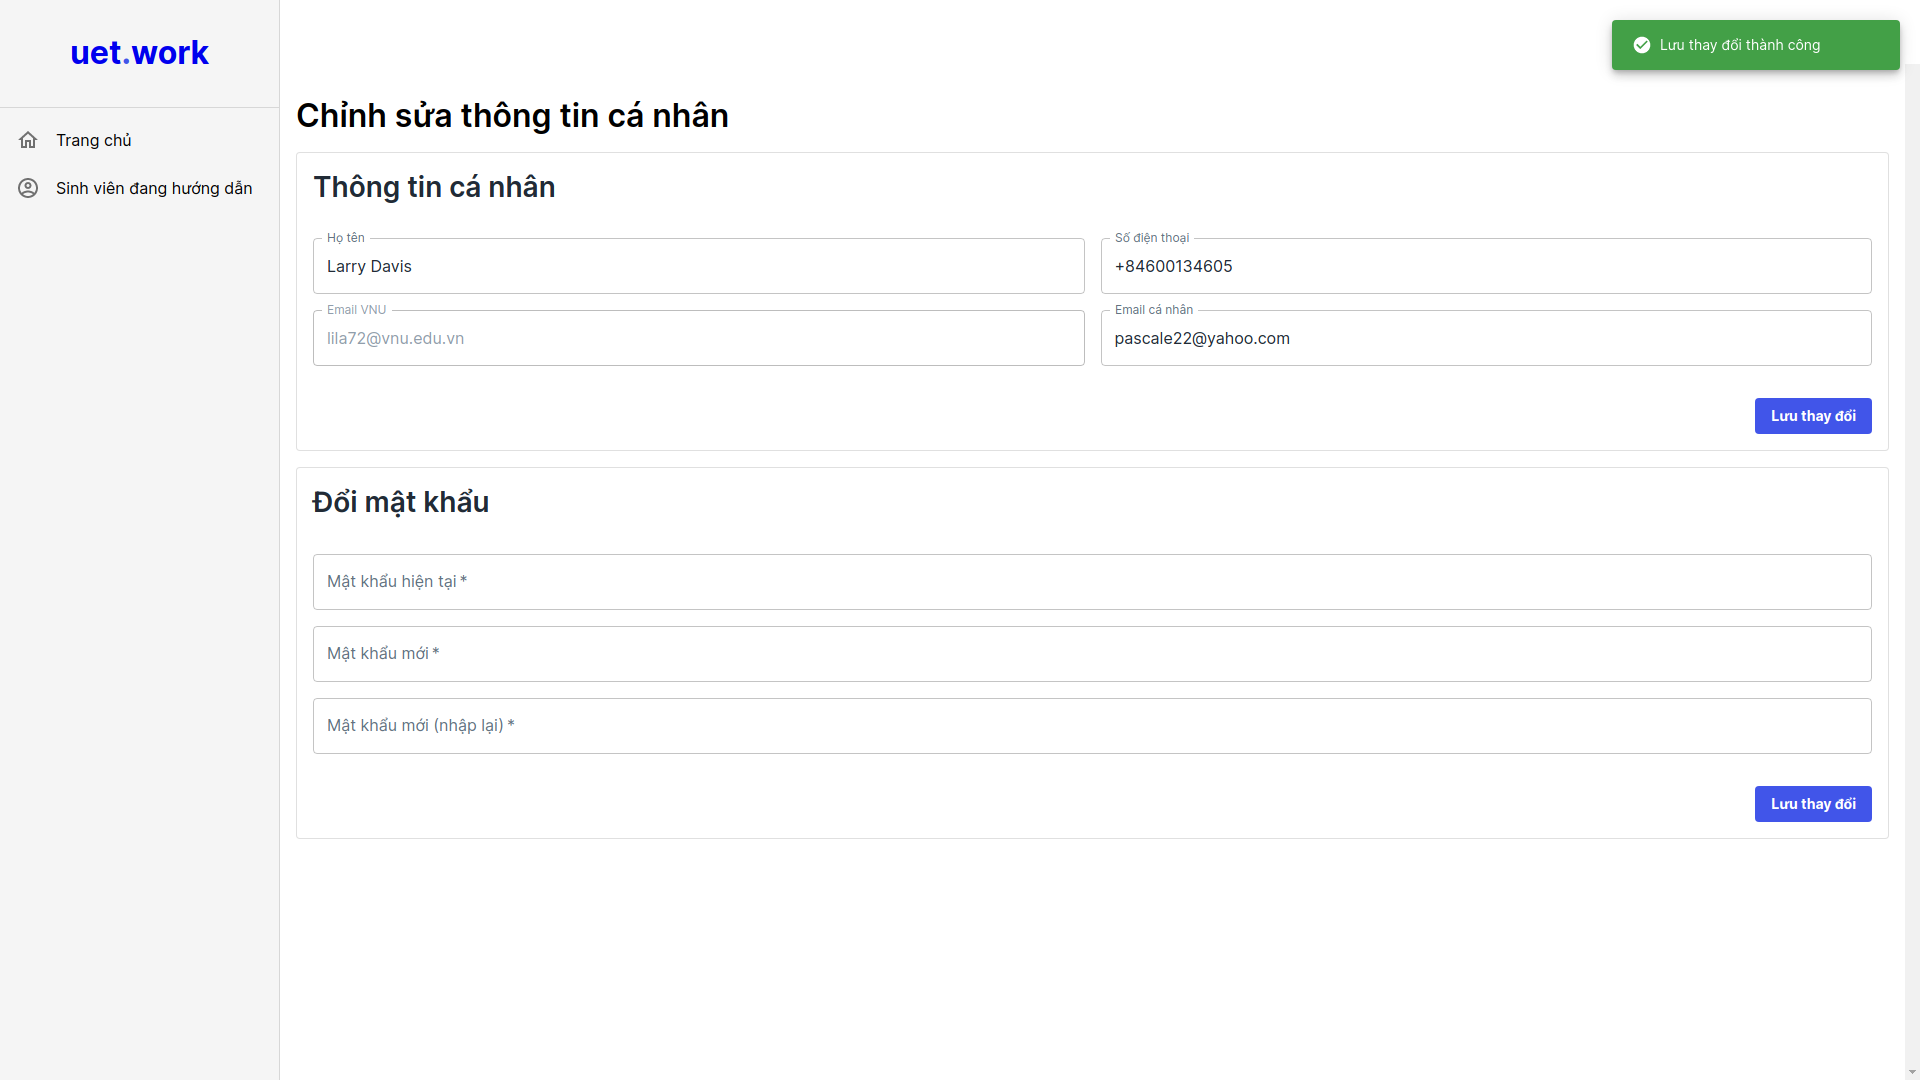
\includegraphics[width=\linewidth]{./images/image52.png}
	\caption{Luồng \emph{Giảng viên thay đổi thông tin cá nhân}: Giảng viên thay đổi thông tin cá nhân}
	\label{fig:lecturer_edit_info}
\end{figure}

\end{document}